\documentclass[12pt, twocolumn]{article}
% font size could be 10pt (default), 11pt or 12 pt
% paper size coulde be letterpaper (default), legalpaper, executivepaper,
% a4paper, a5paper or b5paper
% side coulde be oneside (default) or twoside 
% columns coulde be onecolumn (default) or twocolumn
% graphics coulde be final (default) or draft 
%
% titlepage coulde be notitlepage (default) or titlepage which 
% makes an extra page for title 
% 
% paper alignment coulde be portrait (default) or landscape 
%
% equations coulde be 
%   default number of the equation on the rigth and equation centered 
%   leqno number on the left and equation centered 
%   fleqn number on the rigth and  equation on the left side
%
\usepackage{graphicx}
\title{Reclaiming a Waveguide Switch -- An Adventure In 3D Printing}
\author{Matt Reilly  \\
	kb1vc \\
	}

\date{\today} 
% \date{\today} date coulde be today 
% \date{25.12.00} or be a certain date
% \date{ } or there is no date 
\begin{document}
% Hint: \title{what ever}, \author{who care} and \date{when ever} could stand 
% before or after the \begin{document} command 
% BUT the \maketitle command MUST come AFTER the \begin{document} command! 
\maketitle


\begin{abstract}
  [Engineering] is the art of dong that well with one dollar,
  which any bungler can do with two after a fashion.

  \flushright{Arthur M. Wellington \\
  ``The Economic Theory of \\
  the Location of Railways''}
\end{abstract}

%\tableofcontents % create a table of contens 



\section{Introduction}

Most engineers read Mr. Wellington's dictum as with great pride
that their training has placed them above the run-of-the-mill bungler;
I know that I do.
When it comes to mechanical engineering, however, I am a bungler.
In this case Wellington provides encouragement: it {\em may} be possible
to do what an expert can do for just twice the cost!

And so began my adventures in 3D printing.

\section{Starting Simple}

This article is about reclaiming a WR75 waveguide switch by adapting
a common hobby airplane servo to function as the positioner. It comprises
a relatively simple arduino controller, and a set of plastic parts to
couple the servo to the waveguide slug.

But before we dive in to the construction of the waveguide switch positioner,
it may help to look at a much simpler 3D printing project.

Quite a while back, I bought an HP6289A DC power supply at a hamfest.
It was a real find, but at some point in its checkered past it had
been dropped on its face.  The fall shattered the two fine adjustment
knobs.  These were concentric with the coarse adjustment knobs on two
shafts: one for voltage and the second for current.  For years, the
absence of the knobs was no great annoyance. But one night I decided
that making replacements might be a short and simple project.


In the old days, I'd have scavenged in the scrap box for a nylon rod
or perhaps even an aluminum bar, mounted it in the lathe, turned it down,
bored out the hole for the shaft, tracked a few pieces of swarf while
passing through the living room, found that it didn't quite fit, tried
again... In total, I'd have spent a pleasant hour all together from
looking for bar stock, to vacuuming swarf out of the carpet.

This kind of project really points out the virtues of an inexpensive
3D printer.  No great precision is needed, and the cost of a mistake
is a small amount of material and about 15 minutes of waiting for the
printer to finish. 
In fact, it took two tries to get the design right. (Though had I
been paying attention, it could have been right the first time --
measure twice, print once.) But having the printer in the shack
means that I got through two iterations in less than an hour.
And no metal waste stuck in the carpet. 


\begin{figure}
  \centering
  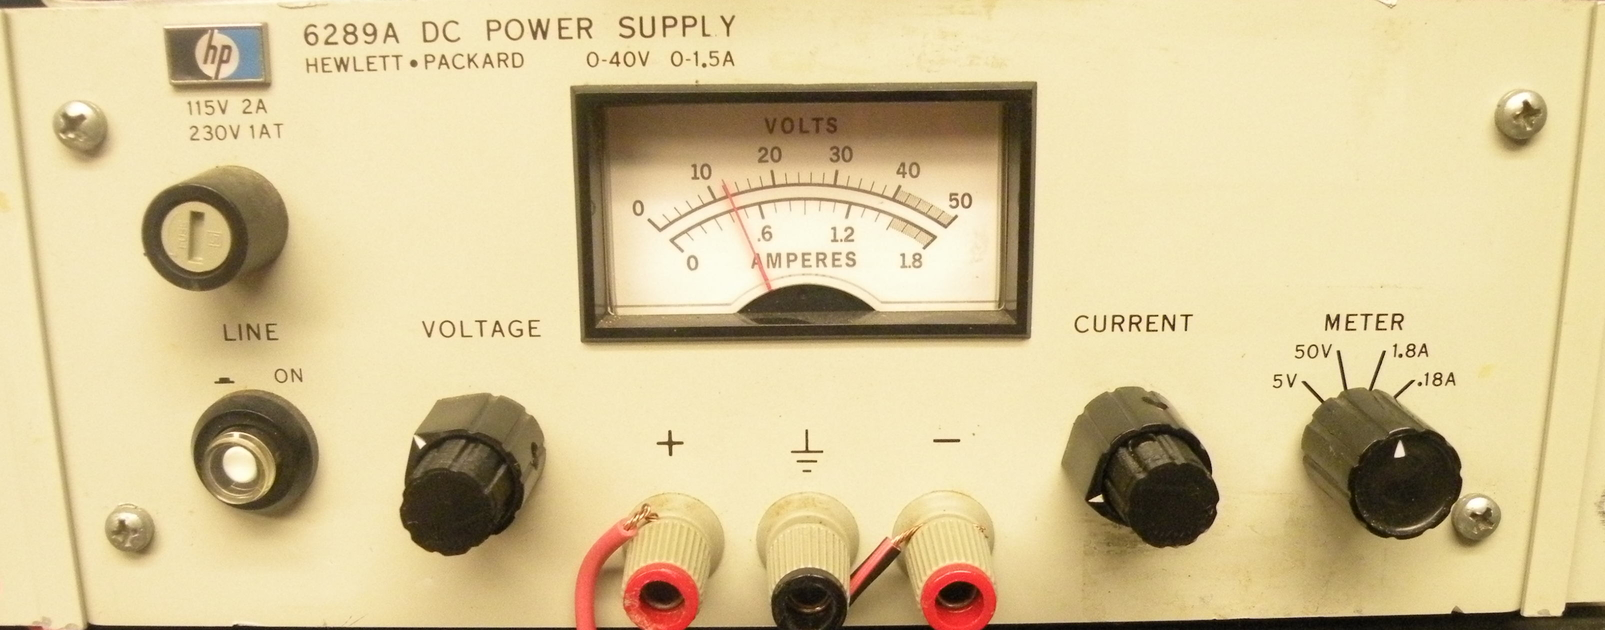
\includegraphics[width=5cm]{PSKnobs.jpg}
  \caption{Replacement power supply knobs in their new home}
\end{figure}

\begin{figure}
  \centering
  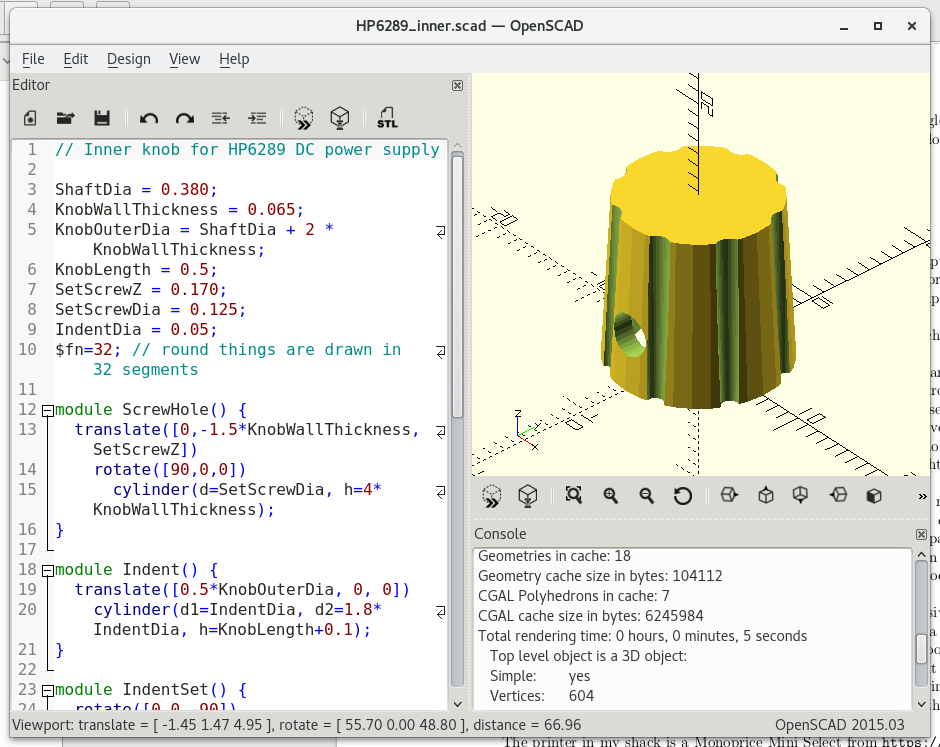
\includegraphics[width=5cm]{PSKnob_OpenSCAD.png}
  \caption{OpenSCAD session showing replacement knob}
\end{figure}




\begin{figure}
  \centering
  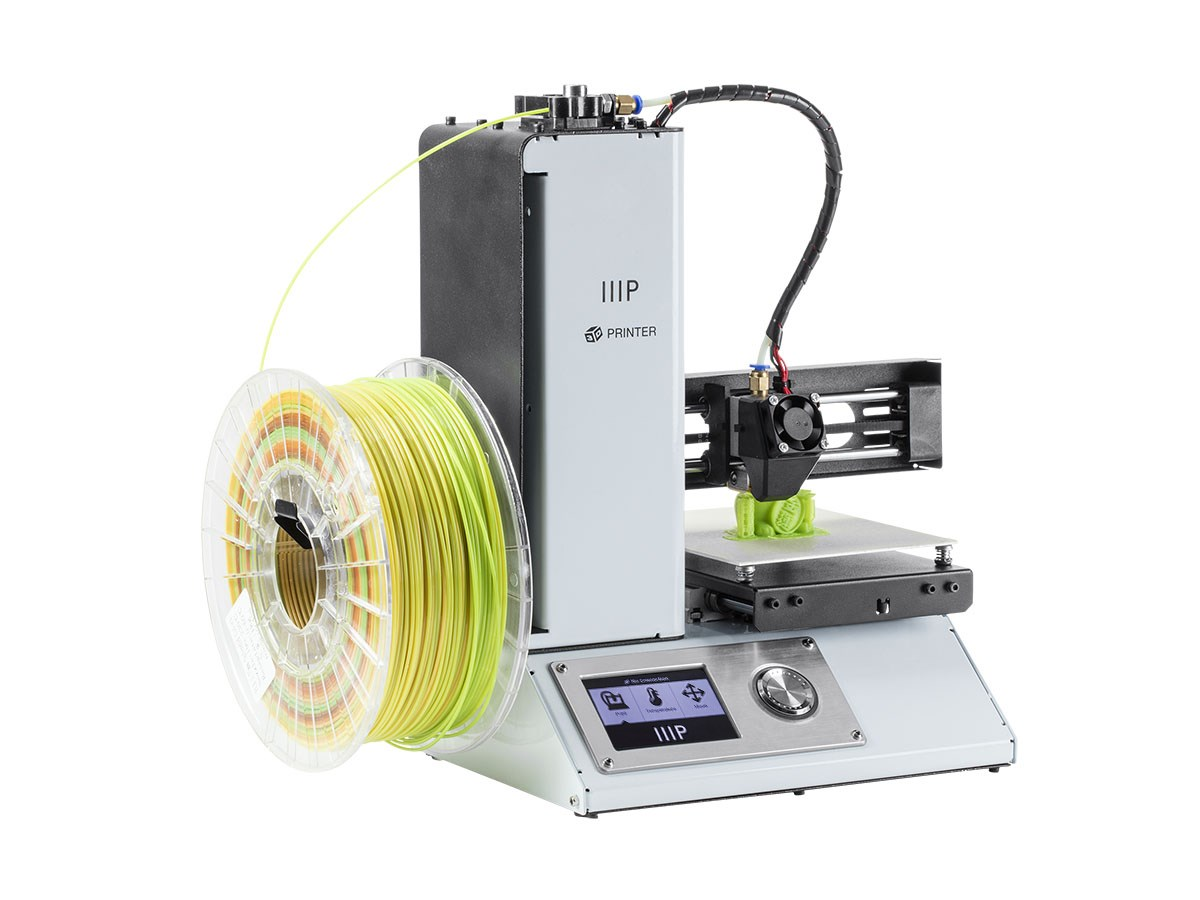
\includegraphics[width=5cm]{MiniSelect3DPrinter.jpg}
  \caption{The Monoprice Mini Select 3D Printer}

  \label{f_printer}
\end{figure}

\begin{figure}
  \centering
  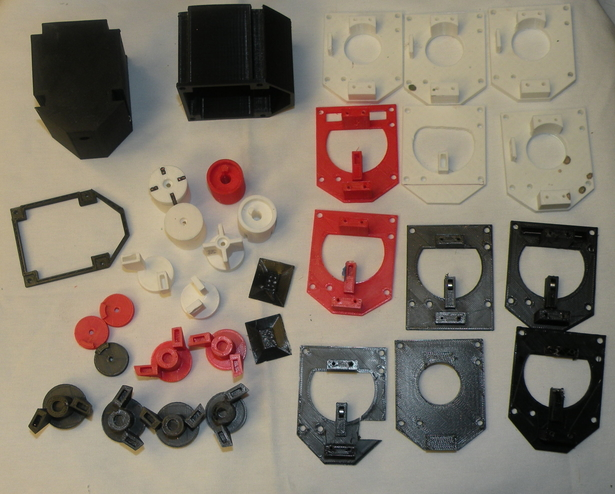
\includegraphics[width=5cm]{TrialAndError1.jpg}
  \caption{Trial and Error Parts}
  \label{f_trial_and_error}
\end{figure}



\end{document}

